%%%%%%%%%%%%%%%%%%%%%%%%%%%%%%%%%%%%%%%%%
% Beamer Presentation
% LaTeX Template
% Version 2.0 (March 8, 2022)
%
% This template originates from:
% https://www.LaTeXTemplates.com
%
% Author:
% Vel (vel@latextemplates.com)
%
% License:
% CC BY-NC-SA 4.0 (https://creativecommons.org/licenses/by-nc-sa/4.0/)
%
%%%%%%%%%%%%%%%%%%%%%%%%%%%%%%%%%%%%%%%%%

%----------------------------------------------------------------------------------------
%	PACKAGES AND OTHER DOCUMENT CONFIGURATIONS
%----------------------------------------------------------------------------------------

\documentclass[
	11pt, % Set the default font size, options include: 8pt, 9pt, 10pt, 11pt, 12pt, 14pt, 17pt, 20pt
	%t, % Uncomment to vertically align all slide content to the top of the slide, rather than the default centered
	%aspectratio=169, % Uncomment to set the aspect ratio to a 16:9 ratio which matches the aspect ratio of 1080p and 4K screens and projectors
]{beamer}

\graphicspath{{Images/}{./}} % Specifies where to look for included images (trailing slash required)

\usepackage{booktabs} % Allows the use of \toprule, \midrule and \bottomrule for better rules in tables

%----------------------------------------------------------------------------------------
%	SELECT LAYOUT THEME
%----------------------------------------------------------------------------------------

% Beamer comes with a number of default layout themes which change the colors and layouts of slides. Below is a list of all themes available, uncomment each in turn to see what they look like.

%\usetheme{default}
%\usetheme{AnnArbor}
%\usetheme{Antibes}
%\usetheme{Bergen}
%\usetheme{Berkeley}
%\usetheme{Berlin}
%\usetheme{Boadilla}
%\usetheme{CambridgeUS}
%\usetheme{Copenhagen}
%\usetheme{Darmstadt}
%\usetheme{Dresden}
%\usetheme{Frankfurt}
%\usetheme{Goettingen}
%\usetheme{Hannover}
%\usetheme{Ilmenau}
%\usetheme{JuanLesPins}
%\usetheme{Luebeck}
\usetheme{Madrid}
%\usetheme{Malmoe}
%\usetheme{Marburg}
%\usetheme{Montpellier}
%\usetheme{PaloAlto}
%\usetheme{Pittsburgh}
%\usetheme{Rochester}
%\usetheme{Singapore}
%\usetheme{Szeged}
%\usetheme{Warsaw}

%----------------------------------------------------------------------------------------
%	SELECT COLOR THEME
%----------------------------------------------------------------------------------------

% Beamer comes with a number of color themes that can be applied to any layout theme to change its colors. Uncomment each of these in turn to see how they change the colors of your selected layout theme.

%\usecolortheme{albatross}
%\usecolortheme{beaver}
%\usecolortheme{beetle}
%\usecolortheme{crane}
%\usecolortheme{dolphin}
%\usecolortheme{dove}
%\usecolortheme{fly}
%\usecolortheme{lily}
%\usecolortheme{monarca}
%\usecolortheme{seagull}
%\usecolortheme{seahorse}
%\usecolortheme{spruce}
%\usecolortheme{whale}
%\usecolortheme{wolverine}

%----------------------------------------------------------------------------------------
%	SELECT FONT THEME & FONTS
%----------------------------------------------------------------------------------------

% Beamer comes with several font themes to easily change the fonts used in various parts of the presentation. Review the comments beside each one to decide if you would like to use it. Note that additional options can be specified for several of these font themes, consult the beamer documentation for more information.

\usefonttheme{default} % Typeset using the default sans serif font
%\usefonttheme{serif} % Typeset using the default serif font (make sure a sans font isn't being set as the default font if you use this option!)
%\usefonttheme{structurebold} % Typeset important structure text (titles, headlines, footlines, sidebar, etc) in bold
%\usefonttheme{structureitalicserif} % Typeset important structure text (titles, headlines, footlines, sidebar, etc) in italic serif
%\usefonttheme{structuresmallcapsserif} % Typeset important structure text (titles, headlines, footlines, sidebar, etc) in small caps serif

%------------------------------------------------

%\usepackage{mathptmx} % Use the Times font for serif text
\usepackage{palatino} % Use the Palatino font for serif text

%\usepackage{helvet} % Use the Helvetica font for sans serif text
\usepackage[default]{opensans} % Use the Open Sans font for sans serif text
%\usepackage[default]{FiraSans} % Use the Fira Sans font for sans serif text
%\usepackage[default]{lato} % Use the Lato font for sans serif text

%----------------------------------------------------------------------------------------
%	SELECT INNER THEME
%----------------------------------------------------------------------------------------

% Inner themes change the styling of internal slide elements, for example: bullet points, blocks, bibliography entries, title pages, theorems, etc. Uncomment each theme in turn to see what changes it makes to your presentation.

%\useinnertheme{default}
\useinnertheme{circles}
%\useinnertheme{rectangles}
%\useinnertheme{rounded}
%\useinnertheme{inmargin}

%----------------------------------------------------------------------------------------
%	SELECT OUTER THEME
%----------------------------------------------------------------------------------------

% Outer themes change the overall layout of slides, such as: header and footer lines, sidebars and slide titles. Uncomment each theme in turn to see what changes it makes to your presentation.

%\useoutertheme{default}
%\useoutertheme{infolines}
%\useoutertheme{miniframes}
%\useoutertheme{smoothbars}
%\useoutertheme{sidebar}
%\useoutertheme{split}
%\useoutertheme{shadow}
%\useoutertheme{tree}
%\useoutertheme{smoothtree}

%\setbeamertemplate{footline} % Uncomment this line to remove the footer line in all slides
%\setbeamertemplate{footline}[page number] % Uncomment this line to replace the footer line in all slides with a simple slide count

%\setbeamertemplate{navigation symbols}{} % Uncomment this line to remove the navigation symbols from the bottom of all slides

%----------------------------------------------------------------------------------------
%	PRESENTATION INFORMATION
%----------------------------------------------------------------------------------------

\title[Computación Evolutiva]{Computación Evolutiva} % The short title in the optional parameter appears at the bottom of every slide, the full title in the main parameter is only on the title page

\subtitle{Una breve introducción} % Presentation subtitle, remove this command if a subtitle isn't required

\author[Luis Alvarado]{Luis Alfredo Alvarado Rodríguez} % Presenter name(s), the optional parameter can contain a shortened version to appear on the bottom of every slide, while the main parameter will appear on the title slide

\institute[]{Distelsa \\ \smallskip \textit{luis.alvarado@distelsa.com.gt}} % Your institution, the optional parameter can be used for the institution shorthand and will appear on the bottom of every slide after author names, while the required parameter is used on the title slide and can include your email address or additional information on separate lines

\date[\today]{Weekly \\ \today} % Presentation date or conference/meeting name, the optional parameter can contain a shortened version to appear on the bottom of every slide, while the required parameter value is output to the title slide

%----------------------------------------------------------------------------------------

\begin{document}

%----------------------------------------------------------------------------------------
%	TITLE SLIDE
%----------------------------------------------------------------------------------------

\begin{frame}
	\titlepage % Output the title slide, automatically created using the text entered in the PRESENTATION INFORMATION block above
\end{frame}

%----------------------------------------------------------------------------------------
%	TABLE OF CONTENTS SLIDE
%----------------------------------------------------------------------------------------

\begin{frame}
	\frametitle{Descripción general de la presentación}
	\tableofcontents
\end{frame}

%----------------------------------------------------------------------------------------
%	PRESENTATION BODY SLIDES
%----------------------------------------------------------------------------------------

\section{Introducción a la Computación Evolutiva}

%------------------------------------------------

\subsection{¿Qué es la Computación Evolutiva?}

\begin{frame}
        \frametitle{Introducción a la Computación Evolutiva}
	\framesubtitle{¿Qué es la Computación Evolutiva?}
	\begin{quote}
		La computación evolutiva es un área de las ciencias de la computación
            que se enfoca al estudio de las propiedades de una serie de metaheurísticas estocásticas (a las cuales se les denomina “Algoritmos Evolutivos”) inspiradas en la teoría de la evolución de las especies formulada por Charles Darwin, según la cual los individuos “más aptos” a su ambiente tienen una mayor probabilidad de sobrevivir. \\
		--- \textbf{Computación Evolutiva, amexcomp.}
	\end{quote}
	
\end{frame}

%------------------------------------------------
\subsection{Historia y Contexto}
\begin{frame}
	\frametitle{Introducción a la Computación Evolutiva}
	\framesubtitle{Historia y Contexto}
	\begin{columns}[c] % The "c" option specifies centered vertical alignment while the "t" option is used for top vertical alignment
		\begin{column}{0.45\textwidth} % Left column width
                La computación evolutiva comenzó a desarrollarse en la década de 1960 como una rama de la inteligencia artificial y la investigación operativa, pero sus raíces conceptuales se basan en la teoría de la evolución de \textbf{Charles Darwin}.
		\end{column}
		\begin{column}{0.5\textwidth} % Right column width
			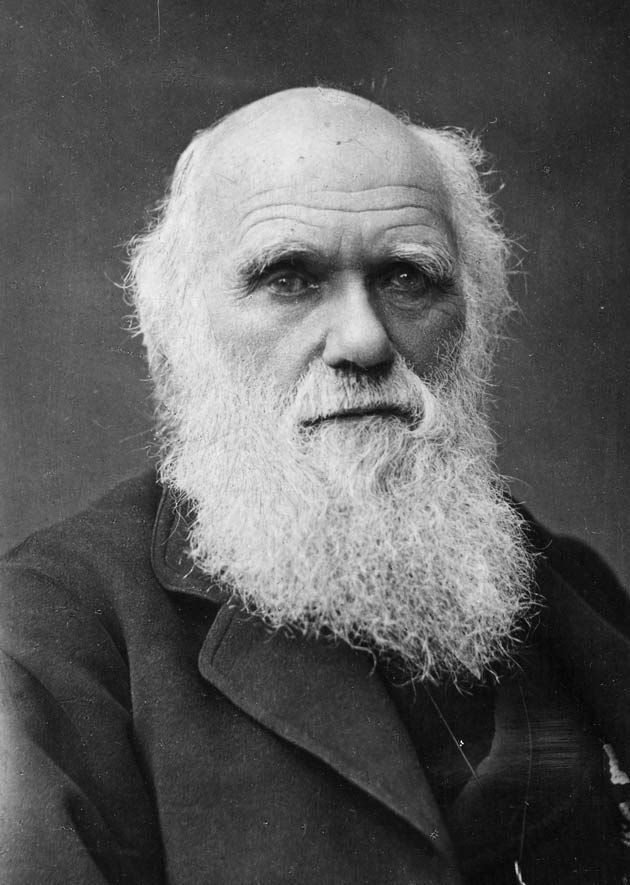
\includegraphics[width=0.8\linewidth]{Images/Charles_Darwin_portrait.jpg}
		\end{column}
	\end{columns}
\end{frame}

\begin{frame}
	\frametitle{Introducción a la Computación Evolutiva}
	\framesubtitle{Historia y Contexto}
	\begin{columns}[c] % The "c" option specifies centered vertical alignment while the "t" option is used for top vertical alignment
		\begin{column}{0.45\textwidth} % Left column width
                \textbf{John Holland} es uno de los pioneros más importantes en este campo. En los años 70, desarrolló el concepto de Algoritmos Genéticos (AG), uno de los primeros y más conocidos enfoques de la computación evolutiva. Los algoritmos genéticos imitan el proceso biológico de la evolución, utilizando procesos de selección, cruzamiento y mutación para mejorar iterativamente las soluciones a un problema.
		\end{column}
		\begin{column}{0.5\textwidth} % Right column width
			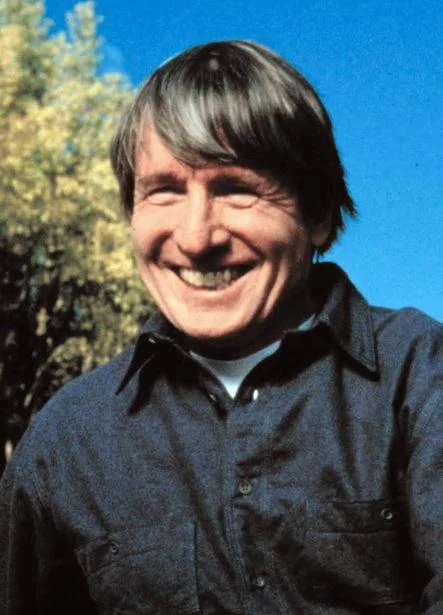
\includegraphics[width=0.8\linewidth]{Images/John_Holland.png}
		\end{column}
	\end{columns}
\end{frame}

%------------------------------------------------
\section{Casos de Uso de la Computación Evolutiva}
\begin{frame}
    \frametitle{Casos de Uso de la Computación Evolutiva}
    \begin{itemize}
        \item \textbf{Optimización de ingeniería}: Diseño de circuitos, rutas óptimas, diseño mecánico, etc.
        \item \textbf{Inteligencia artificial en juegos}: Ejemplo de criaturas evolutivas en simuladores de videojuegos.
        \item \textbf{Machine Learning}: Evolución de hiperparámetros en redes neuronales y otros modelos.
        \item \textbf{Investigación científica}: Aplicación en biología computacional (por ejemplo, simulación de evolución de poblaciones).
        \item \textbf{Economía y finanzas}: Uso en la optimización de carteras de inversión o la simulación de mercados.
    \end{itemize}
    
\end{frame}

%------------------------------------------------
\section{Fundamentos Teóricos de la Computación Evolutiva}
\subsection{Algoritmos Evolutivos (AEs)}
\begin{frame}
	\frametitle{Fundamentos Teóricos de la Computación Evolutiva}
	\framesubtitle{Algoritmos Evolutivos (AEs)}
        Los \textbf{algoritmos evolutivos (AEs)} son modelos computacionales que simulan procesos evolutivos para resolver problemas de optimización y búsqueda. Se basan en los mecanismos de la evolución biológica, como la selección natural, el cruzamiento y la mutación, y se utilizan cuando no existe un método determinístico que pueda encontrar la solución óptima de manera eficiente. Los AEs son útiles en problemas donde el espacio de soluciones es vasto y las soluciones óptimas no están claramente definidas.
\end{frame}

\begin{frame}
	\frametitle{Fundamentos Teóricos de la Computación Evolutiva}
	\framesubtitle{Inspiración biológica}
        \begin{center}
            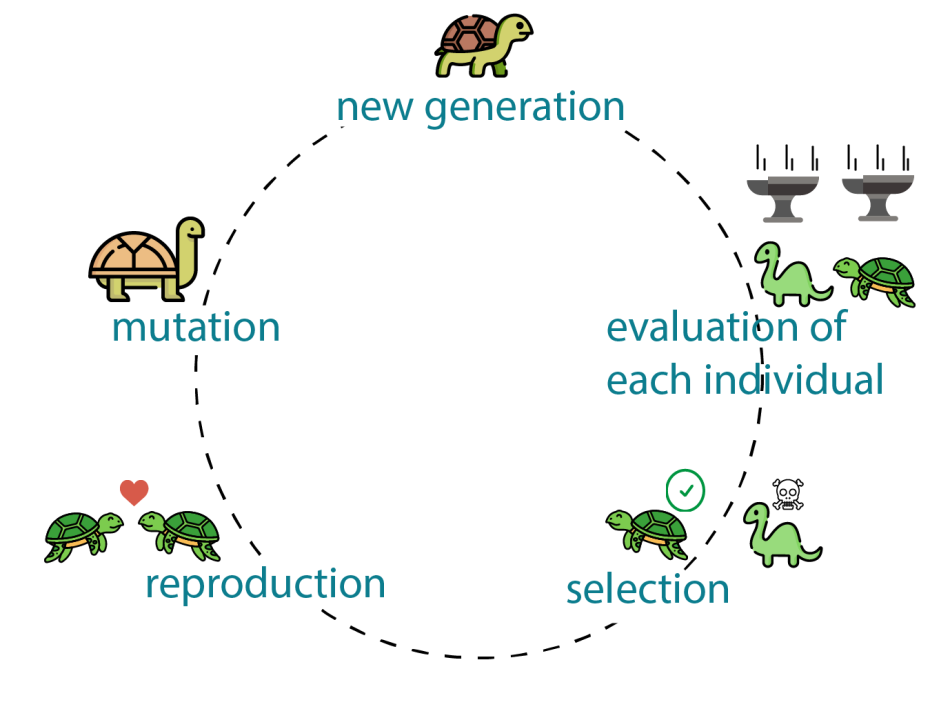
\includegraphics[width=0.8\linewidth]{Images/evolution.png}
        \end{center}
\end{frame}

%------------------------------------------------
\subsection{Tipos de Algoritmos Evolutivos}
\begin{frame}
    \frametitle{Fundamentos Teóricos de la Computación Evolutiva}
    \framesubtitle{Tipos de Algoritmos Evolutivos}
    \begin{enumerate}
        \item \textbf{Algoritmos Genéticos (AGs):}
        
        Los \textbf{algoritmos genéticos (AGs)} son quizás el tipo más conocido de algoritmos evolutivos. Inspirados en los mecanismos de la genética biológica, se enfocan en el cruce y la mutación de genes (representación binaria o de otro tipo) para generar nuevas soluciones.
        
        \begin{itemize}
            \item Usan una población de cromosomas (individuos) que se combinan y mutan para buscar mejores soluciones.
            \item Aplicaciones: Optimización de rutas, problemas de diseño, inteligencia artificial en videojuegos.
        \end{itemize}
    \end{enumerate}
\end{frame}

\begin{frame}
    \frametitle{Fundamentos Teóricos de la Computación Evolutiva}
    \framesubtitle{Tipos de Algoritmos Evolutivos}
    \begin{enumerate}
    \setcounter{enumi}{1}
        \item \textbf{Estrategias Evolutivas (ESs):}
        
        Las \textbf{estrategias evolutivas (ESs)}, desarrolladas por Rechenberg y Schwefel, se centran en la evolución de parámetros continuos y son especialmente útiles para resolver problemas de optimización numérica. Las ESs se diferencian de los algoritmos genéticos en que hacen más hincapié en la mutación que en el cruzamiento.
        
        \begin{itemize}
            \item Utilizan la mutación como principal operador de variación, y la recombinación (cruzamiento) se usa de manera opcional o limitada.
            \item Aplicaciones: Optimización de parámetros en sistemas mecánicos, diseño de estructuras, calibración de sistemas de control.
        \end{itemize}
    \end{enumerate}
\end{frame}

\begin{frame}
    \frametitle{Fundamentos Teóricos de la Computación Evolutiva}
    \framesubtitle{Tipos de Algoritmos Evolutivos}
    \begin{enumerate}
    \setcounter{enumi}{2}
        \item \textbf{Programación Genética (GP):}
        
        La \textbf{programación genética (GP)} es un tipo de algoritmo evolutivo en el que los individuos son programas de computadora. Los programas se evalúan en función de su capacidad para resolver un problema determinado, y luego evolucionan a través de cruces y mutaciones para generar mejores programas.
        
        \begin{itemize}
            \item En lugar de soluciones representadas como vectores o cadenas de bits, en GP los individuos son estructuras de programas, como árboles de expresiones.
            \item Aplicaciones: Automatización de código, diseño de algoritmos, aprendizaje automático.
        \end{itemize}
    \end{enumerate}
\end{frame}
%------------------------------------------------
\subsection{Proceso General de un Algoritmo Evolutivo}
\begin{frame}
    \frametitle{Fundamentos Teóricos de la Computación Evolutiva}
    \framesubtitle{Proceso General de un Algoritmo Evolutivo}
    \begin{enumerate}
        \item \textbf{Inicialización: Generación de la población inicial}
        
        El primer paso en un algoritmo evolutivo es generar una población inicial de individuos. Cada uno de estos individuos representa una posible solución al problema, y puede codificarse como una cadena de datos (por ejemplo, una secuencia binaria, un vector de números reales, o incluso un programa en el caso de la programación genética).
        
        \begin{itemize}
            \item \textbf{Población inicial}: Puede ser generada de manera aleatoria o usando algún conocimiento previo del problema para mejorar las soluciones iniciales.
            \item \textbf{Tamaño de la población}: El número de individuos en la población varía según el problema y afecta el rendimiento del algoritmo. Poblaciones más grandes permiten explorar más el espacio de búsqueda, pero aumentan el costo computacional.
        \end{itemize}
    \end{enumerate}
\end{frame}

\begin{frame}
    \frametitle{Fundamentos Teóricos de la Computación Evolutiva}
    \framesubtitle{Proceso General de un Algoritmo Evolutivo}
    \begin{enumerate}
    \setcounter{enumi}{1}
        \item \textbf{Evaluación: Aplicación de la función de fitness}
        
        Una vez generada la población inicial, se evalúa a cada individuo aplicando la \textbf{función de fitness}. Esta función mide la calidad de cada solución, determinando qué tan "buena" o "adecuada" es en comparación con otras soluciones. Los individuos con un mejor valor de fitness tendrán mayor probabilidad de ser seleccionados para la siguiente generación.
        
        \begin{itemize}
            \item \textbf{Función de fitness}: Dependiendo del problema, puede ser una medida directa (por ejemplo, la distancia mínima en un problema de rutas) o una evaluación basada en una simulación.
            \item \textbf{Evaluación cuantitativa}: Asigna un valor numérico que refleja el rendimiento o la calidad de la solución.
        \end{itemize}
    \end{enumerate}
\end{frame}

\begin{frame}
    \frametitle{Fundamentos Teóricos de la Computación Evolutiva}
    \framesubtitle{Proceso General de un Algoritmo Evolutivo}
    \begin{enumerate}
    \setcounter{enumi}{2}
        \item \textbf{Selección: Supervivencia del más apto}
        
        En este paso, se eligen los individuos que pasarán a la siguiente generación. Los mejores individuos (aquellos con mayor fitness) tienen una mayor probabilidad de ser seleccionados, lo que refleja la idea de la "supervivencia del más apto". Existen diferentes métodos para la selección:
        
        \begin{itemize}
            \item \textbf{Método de la ruleta}: Los individuos se seleccionan de manera probabilística, donde la probabilidad de ser seleccionado es proporcional a su valor de fitness.
            \item \textbf{Torneo}: Un subconjunto aleatorio de individuos compite, y el ganador (con mejor fitness) es seleccionado.
            \item \textbf{Selección por ranking}: Los individuos se ordenan según su fitness, y se seleccionan en función de su posición en el ranking.
        \end{itemize}
    \end{enumerate}
\end{frame}

\begin{frame}
    \frametitle{Fundamentos Teóricos de la Computación Evolutiva}
    \framesubtitle{Proceso General de un Algoritmo Evolutivo}
    \begin{enumerate}
    \setcounter{enumi}{3}
        \item \textbf{Cruzamiento y mutación: Generación de nuevas soluciones}
        
        \textbf{Cruzamiento}: Después de seleccionar los individuos, se combina la información genética de dos padres para generar uno o más hijos.
        
        \begin{itemize}
            \item \textbf{Cruzamiento de un punto}: Se selecciona un punto aleatorio en los cromosomas de los padres, y se intercambian las partes después de ese punto.
            \item \textbf{Cruzamiento uniforme}: Cada gen se intercambia entre los padres con una probabilidad fija.
        \end{itemize}
        
        \textbf{Mutación}: Tras el cruzamiento, algunos individuos sufren pequeñas modificaciones aleatorias. La mutación es clave para mantener la diversidad en la población y explorar nuevas áreas del espacio de soluciones.
        
        \begin{itemize}
            \item \textbf{Mutación puntual}: Cambio de un valor o bit en un individuo.
            \item \textbf{Mutación por desplazamiento}: Se cambia una parte del cromosoma por otra con un valor diferente.
        \end{itemize}
    \end{enumerate}
\end{frame}

\begin{frame}
    \frametitle{Fundamentos Teóricos de la Computación Evolutiva}
    \framesubtitle{Proceso General de un Algoritmo Evolutivo}
    \begin{enumerate}
    \setcounter{enumi}{4}
        \item \textbf{Iteración: Repetición del ciclo hasta encontrar la solución óptima}
        
        El proceso de evaluación, selección, cruzamiento y mutación se repite durante varias generaciones. En cada iteración, la población evoluciona, mejorando sus soluciones hasta cumplir con uno de los siguientes criterios de parada:
        
        \begin{itemize}
            \item \textbf{Número máximo de generaciones}: El algoritmo se detiene después de ejecutar un número fijo de iteraciones.
            \item \textbf{Convergencia}: Si no se observan mejoras significativas en la población durante varias generaciones, se puede suponer que se ha alcanzado una solución cercana al óptimo.
            \item \textbf{Criterio de fitness}: El algoritmo se detiene cuando se alcanza un valor de fitness predefinido que satisface las expectativas.
        \end{itemize}
    \end{enumerate}
\end{frame}

%------------------------------------------------
\subsection{Representación algorítmica}
\begin{frame}
	\frametitle{Fundamentos Teóricos de la Computación Evolutiva}
	\framesubtitle{Representación algorítmica}
        \begin{center}
            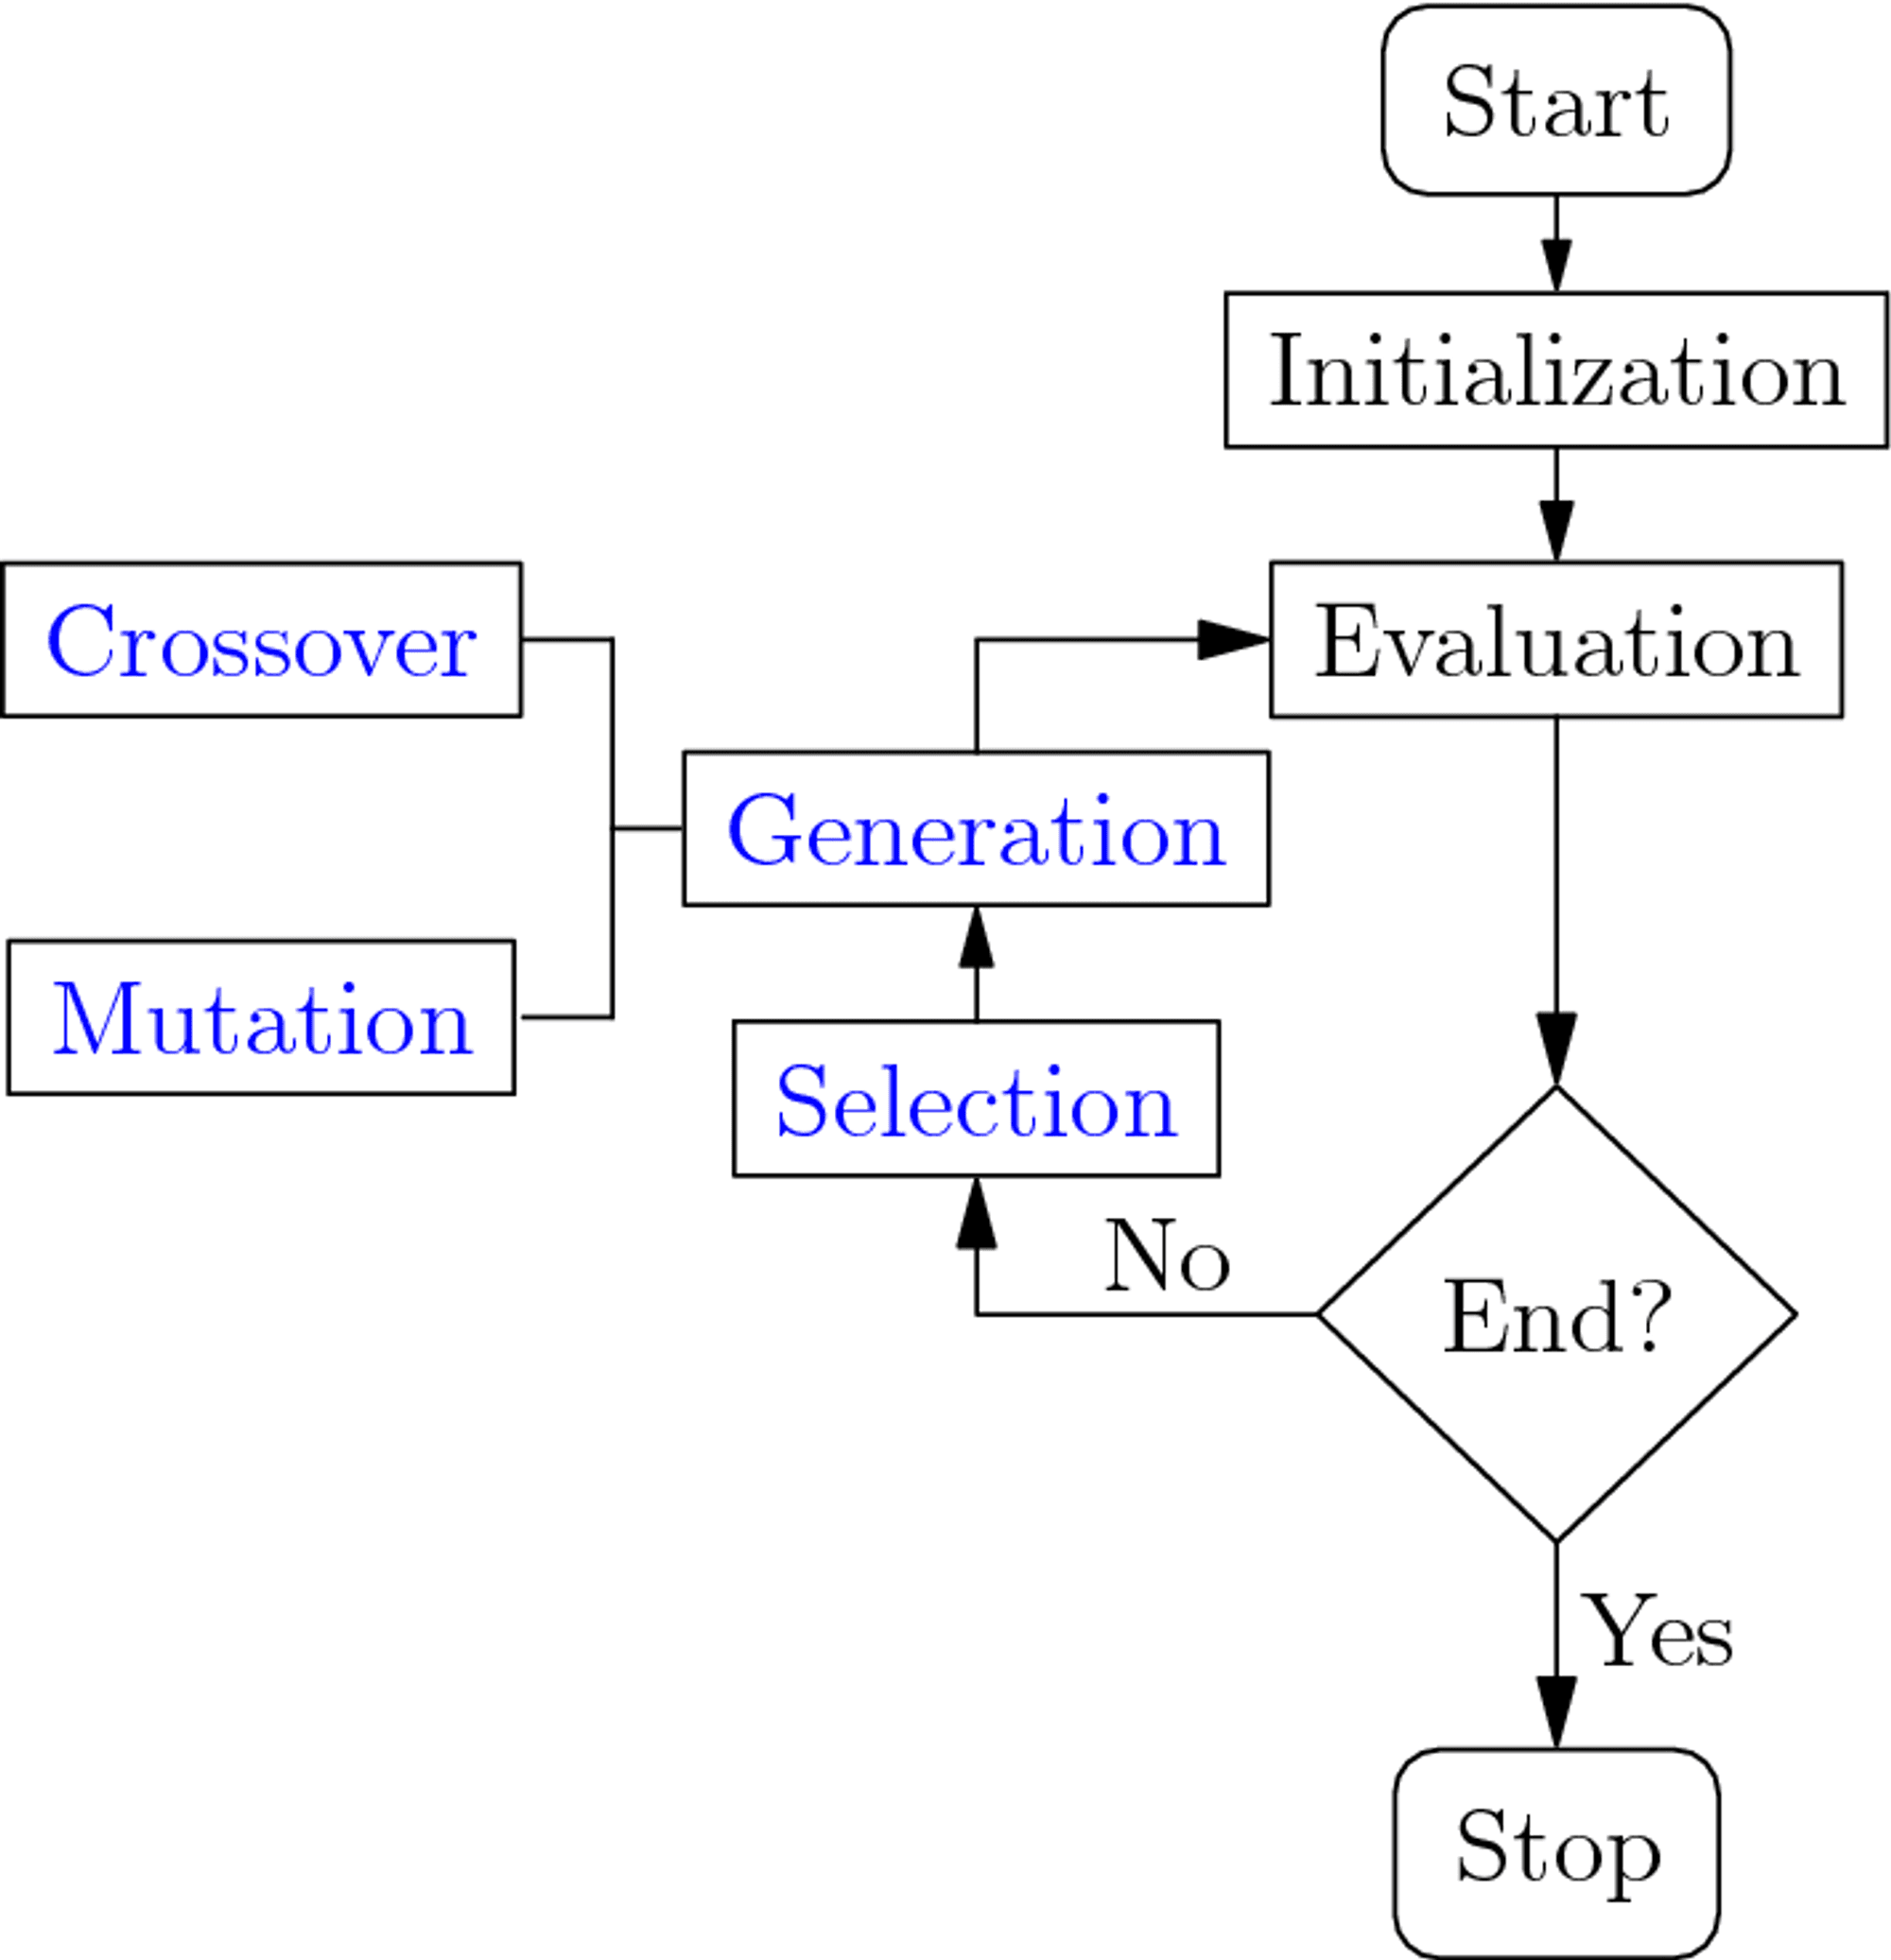
\includegraphics[width=0.5\linewidth]{Images/Genetic_Algorithm_in_AI_Workflow_f216628d31.png}
        \end{center}
\end{frame}

\begin{frame}
	\frametitle{Fundamentos Teóricos de la Computación Evolutiva}
	\framesubtitle{Representación algorítmica}
        \begin{center}
            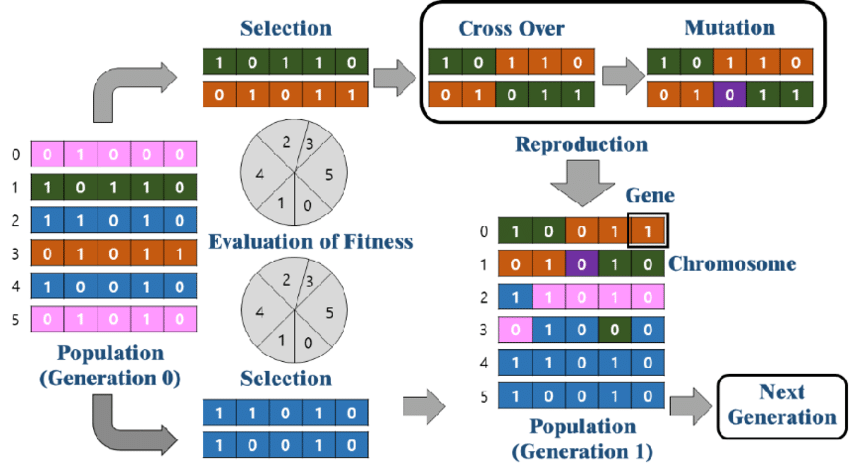
\includegraphics[width=0.8\linewidth]{Images/Genetic-selection-method-using-genetic-algorithm.png}
        \end{center}
\end{frame}

\begin{frame}
	\frametitle{Fundamentos Teóricos de la Computación Evolutiva}
	\framesubtitle{Representación algorítmica}
        \begin{center}
            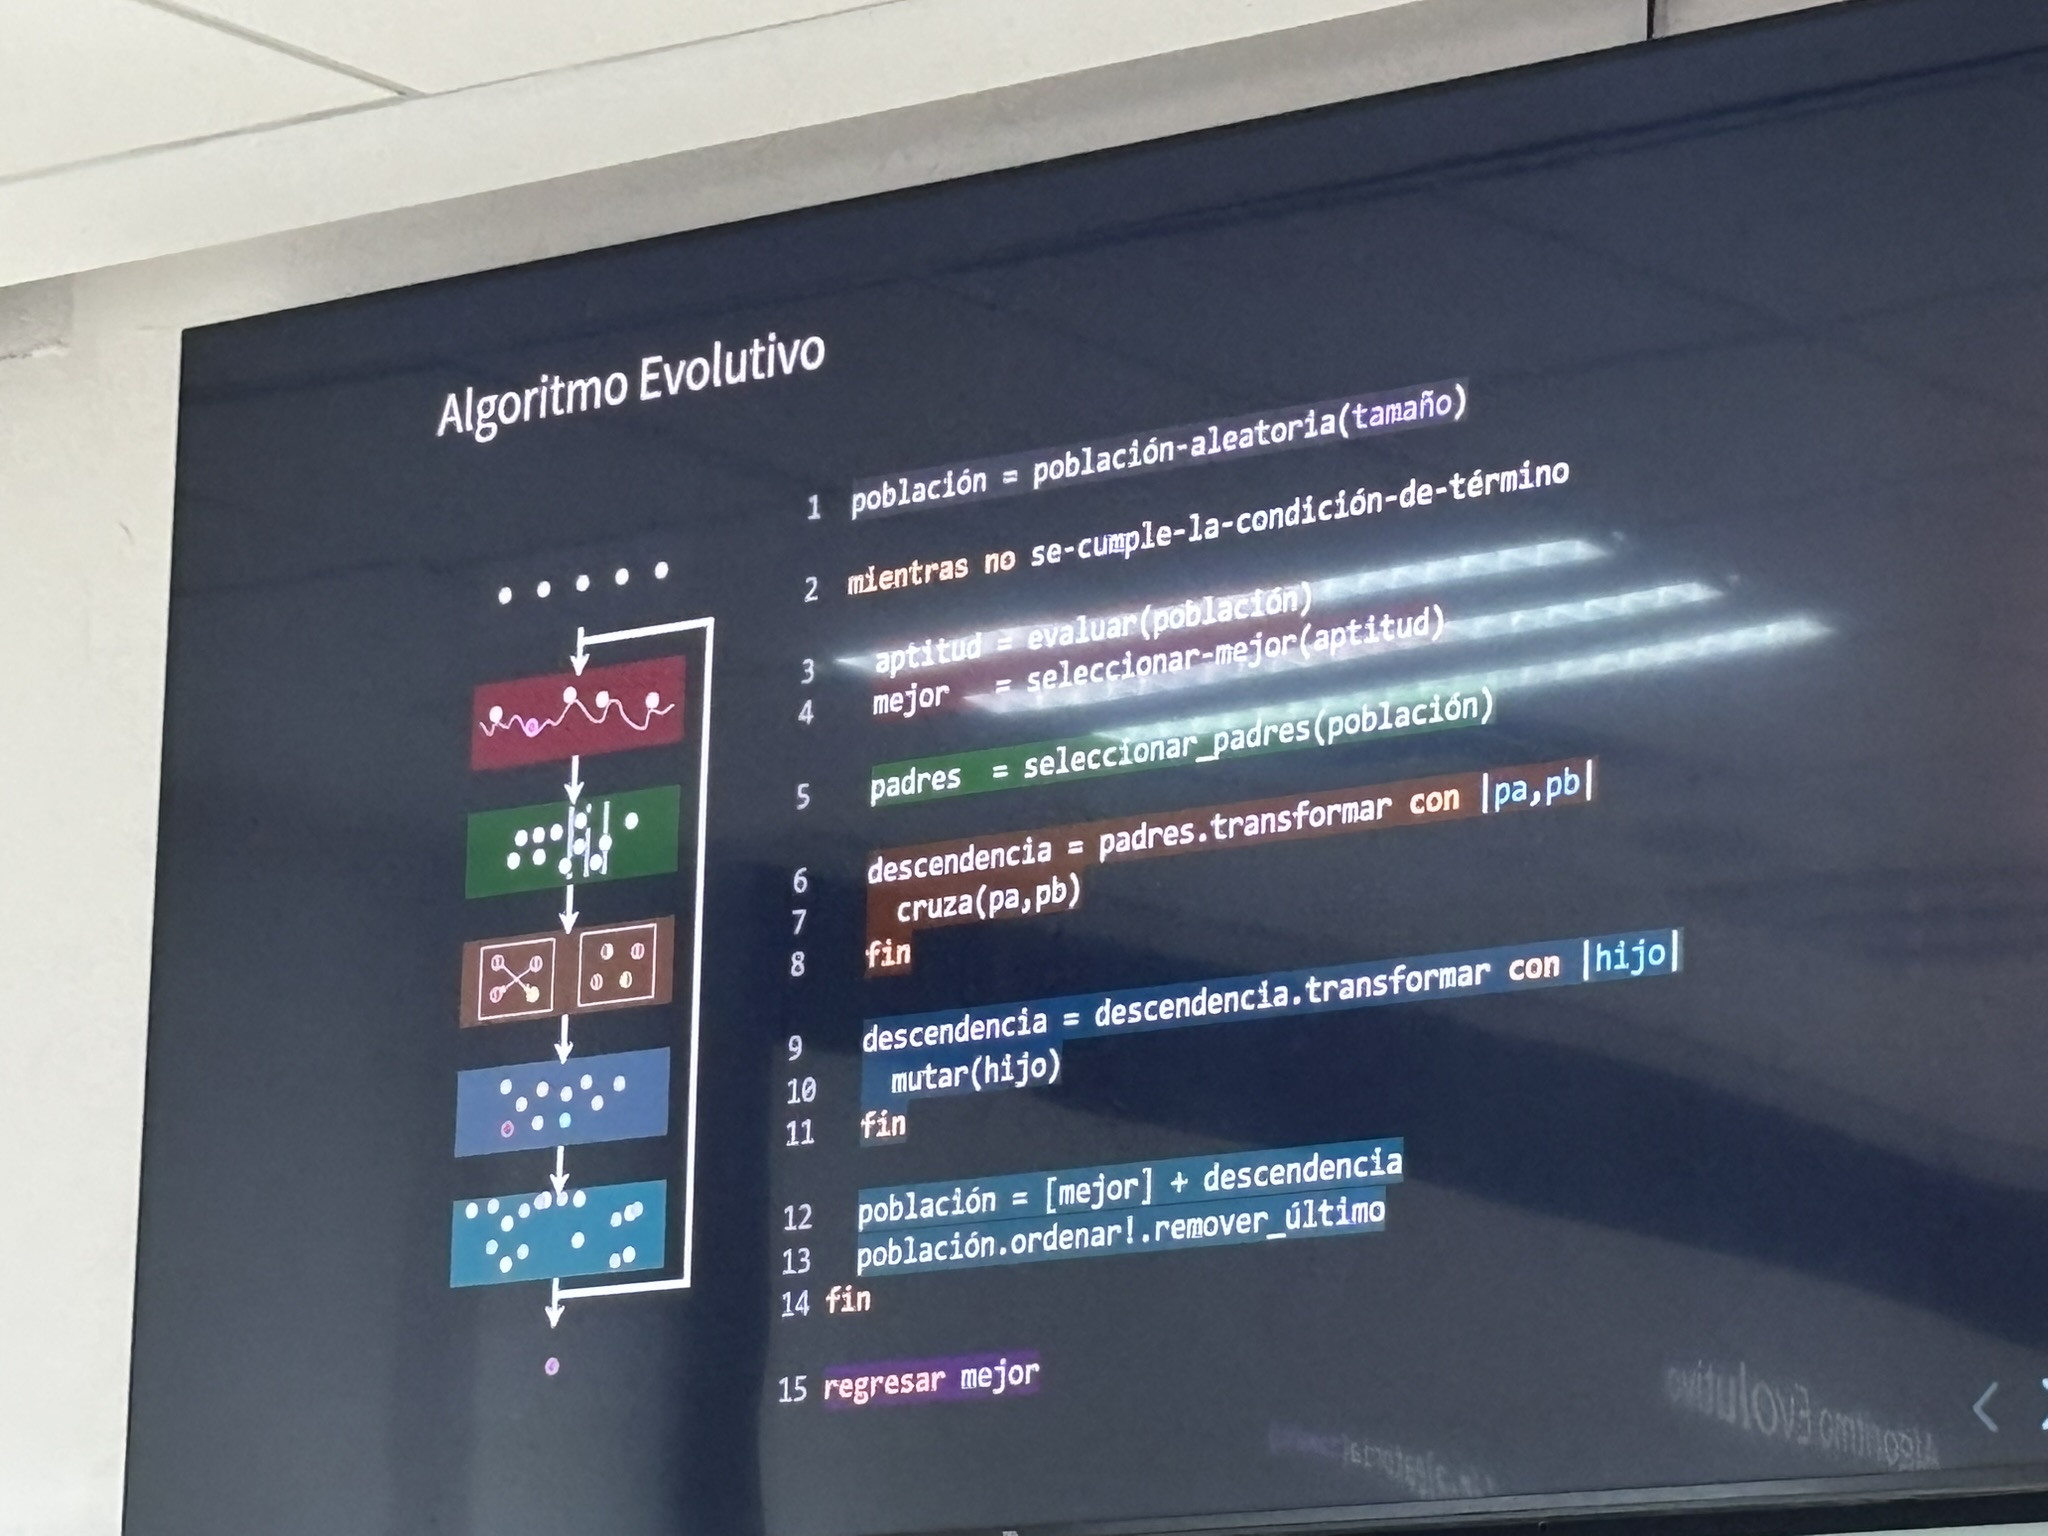
\includegraphics[width=0.8\linewidth]{Images/17AF6DCD-F830-42A0-95A0-B05FA1DE91B7_1_102_o.jpeg}
        \end{center}
\end{frame}

%------------------------------------------------
\section{Ventajas y Desventajas de la Computación Evolutiva}
\begin{frame}
    \frametitle{Ventajas y Desventajas de la Computación Evolutiva}
    \begin{itemize}
        \item \textbf{Ventajas}:
        \begin{itemize}
            \item Versatilidad para resolver problemas complejos.
            \item Flexibilidad y capacidad de adaptación.
            \item Funciona bien con problemas de optimización de múltiples objetivos.
        \end{itemize}
        \item \textbf{Desventajas}:
        \begin{itemize}
            \item Alto costo computacional.
            \item Poca garantía de alcanzar la solución óptima (puede quedarse en óptimos locales).
            \item Requiere ajuste manual de parámetros para un buen rendimiento.
        \end{itemize}
    \end{itemize}
\end{frame}
%------------------------------------------------
\section{Ejercicio Práctico: Algoritmo Evolutivo Simple}
\begin{frame}
    \frametitle{Ejercicio Práctico: Algoritmo Evolutivo Simple}
    \framesubtitle{Descripción del problema}
    \begin{block}{Enunciado}
        Optimizar la función:
        \begin{equation*}
            f(x) = -(x - 3)^2 + 10
        \end{equation*}
    \end{block}
\end{frame}
\begin{frame}
    \frametitle{Ejercicio Práctico: Algoritmo Evolutivo Simple}
    \framesubtitle{Análisis inicial}
    \begin{center}
        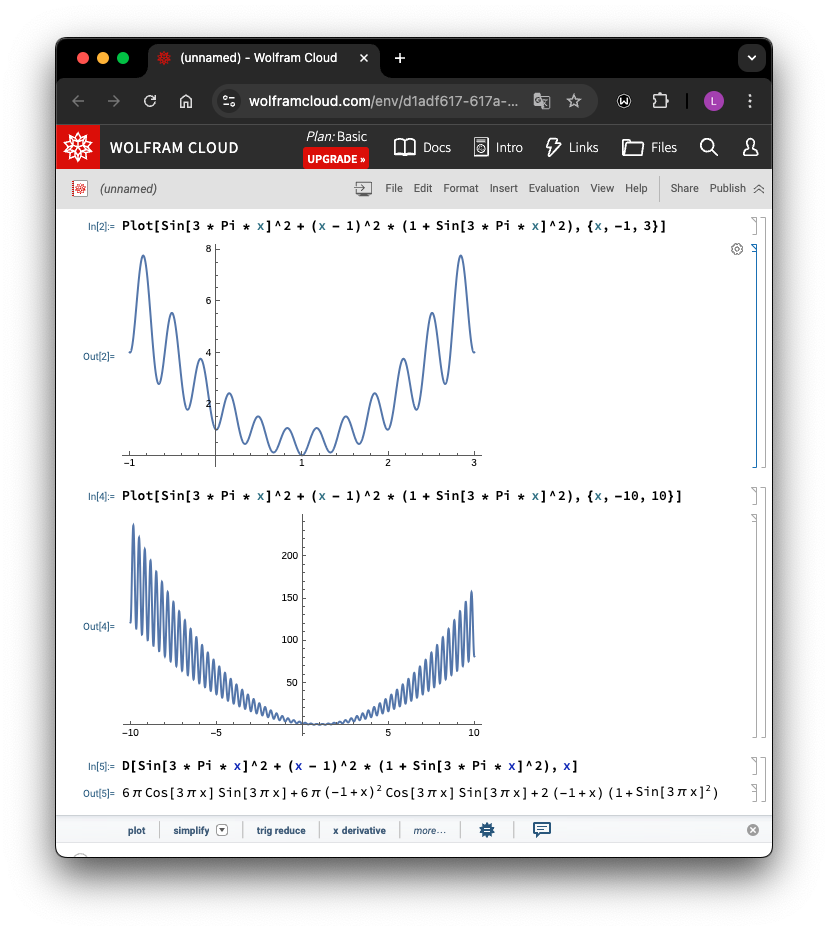
\includegraphics[width=0.6\linewidth]{Images/Captura de pantalla 2024-10-23 a la(s) 6.45.02 p. m..png}
    \end{center}
\end{frame}
%------------------------------------------------

\begin{frame}
    \frametitle{Referencias}
    
    \begin{thebibliography}{99}
        \footnotesize
        
        \bibitem[Coello Coello, 2019]{p3}
            Carlos Artemio Coello Coello (Editor) (2019) \\
            \emph{Computaci\'on Evolutiva}, Segunda Edici\'on, Academia Mexicana de Computaci\'on, A.C. \\
            ISBN: 978-607-97357-9-1 \\
            Disponible en: \href{https://amexcomp.mx/media/publicaciones/comp-evolutiva.pdf}{comp-evolutiva.pdf}

        \bibitem[Ansari, 2020]{p4}
            Sakil Ansari (2020) \\
            \emph{Hyperparameter tuning in Random Forest Classifier using genetic algorithm} \\
            Disponible en: \href{https://sakilansari4.medium.com/hyperparameter-tuning-in-random-forest-classifier-using-genetic-algorithm-ae582ae6655c}{Medium Article}

        \bibitem[Arenas, 2021]{p5}
            Rodrigo Arenas (2021) \\
            \emph{Tune Your Scikit-learn Model Using Evolutionary Algorithms} \\
            Publicado en: Towards Data Science \\
            Disponible en: \href{https://towardsdatascience.com/tune-your-scikit-learn-model-using-evolutionary-algorithms-30538248ac16}{Towards Data Science}

        \bibitem[Udemy, 2023]{p6}
            Udemy (2023) \\
            \emph{Genetic Algorithm Courses on Udemy} \\
            Disponible en: \href{https://www.udemy.com/courses/search/?src=ukw&q=Genetic+Algorithm}{Cursos en Udemy}
    \end{thebibliography}
\end{frame}




%----------------------------------------------------------------------------------------
%	CLOSING SLIDE
%----------------------------------------------------------------------------------------

\begin{frame}[plain]
	\begin{center}
		{\Huge Fin}
		
		\bigskip\bigskip
		
		{\LARGE ¿Preguntas? ¿Comentarios?}
	\end{center}
\end{frame}

%----------------------------------------------------------------------------------------

\end{document} 